\documentclass[12pt]{article}

% -------------------------
% PAQUETES NECESARIOS
% -------------------------
\usepackage[utf8]{inputenc}
\usepackage[T1]{fontenc}
\usepackage{titlesec}
\usepackage{fancyhdr}
\usepackage{graphicx}
\usepackage{listings}
\usepackage{xcolor}
\usepackage{geometry}
\usepackage[spanish]{babel}
\usepackage{hyperref}
\usepackage{graphicx}
\usepackage{booktabs} % Para líneas profesionales (\toprule, \midrule, \bottomrule)
\usepackage{multirow} % Para agrupar celdas verticales

% -------------------------
% CONFIGURACIÓN DE PÁGINA
% -------------------------
\geometry{margin=2.5cm}

% Fuente tipo Times New Roman equivalente
\usepackage{mathptmx}

% Interlineado sencillo (por defecto en LaTeX)

% -------------------------
% CONFIGURACIÓN DE ENCABEZADO Y PIE
% -------------------------
\pagestyle{fancy}
\fancyhf{}

\fancyhead[L]{Multiprogramación paralela}
\fancyhead[R]{2026/2027}

\fancyfoot[L]{Andrey, Abdellah} % <-- EDITAR
\fancyfoot[R]{\thepage}

\renewcommand{\headrulewidth}{0.4pt}
\renewcommand{\footrulewidth}{0.4pt}


\usepackage{listings}
\usepackage{xcolor}

% --- Colores generales ---
\definecolor{mGreen}{rgb}{0,0.6,0}
\definecolor{mGray}{rgb}{0.5,0.5,0.5}
\definecolor{mPurple}{rgb}{0.58,0,0.82}
\definecolor{bgC}{rgb}{0.98,0.98,0.98}
\definecolor{bgValgrind}{rgb}{0.93,0.93,0.93}

% --- ESTILO 1: Para Código C ---
\lstdefinestyle{EstiloC}{
    backgroundcolor=\color{bgC},   
    commentstyle=\color{mGreen}\itshape,
    keywordstyle=\color{magenta}\bfseries,
    numberstyle=\tiny\color{mGray},
    stringstyle=\color{mPurple},
    basicstyle=\ttfamily\footnotesize,
    breakatwhitespace=false,         
    breaklines=true,                 % ¡Evita que el código se salga por la derecha!
    captionpos=b,                    
    keepspaces=true,                 
    numbers=left,                    
    numbersep=8pt,                  
    showstringspaces=false,
    tabsize=4,
    language=C,
    frame=single,                    
    rulecolor=\color{mGray!30}
}

% --- ESTILO 2: Para trazas/logs de Valgrind ---
\lstdefinestyle{EstiloValgrind}{
    backgroundcolor=\color{bgValgrind},
    basicstyle=\ttfamily\scriptsize, % Letra ligeramente más pequeña para trazas anchas
    breakatwhitespace=false,
    breaklines=true,                 % ¡Evita que los reportes de Valgrind se corten!
    captionpos=b,
    frame=single,
    numbers=none,                    % Sin números de línea para logs de terminal
    showstringspaces=false,
    language={},                     % Sin resaltado de sintaxis de lenguaje
    rulecolor=\color{mGray!50}
}


% -------------------------
% INICIO DEL DOCUMENTO
% -------------------------
\begin{document}

% =========================
% PORTADA
% =========================
\thispagestyle{empty}



% Bloque arriba a la derecha
\begin{flushright}
Abdellah Bensaidi, Souri 1.3\\
Morales Vicuña, Andrey 1.1\\
Asignatura: Multiprogramación paralela \\
Grupo: 1 \\
%  Subgrupo: 1.1 \\

\end{flushright}

\vfill

% Imagen centrada
\begin{center}

\includegraphics[width=0.4\textwidth]{sello.png}
\end{center}

\vfill

% Fecha abajo
\begin{center}
\today
\end{center}

\newpage

\newpage
\tableofcontents
\newpage

\begin{figure}[htbp]
    \centering
    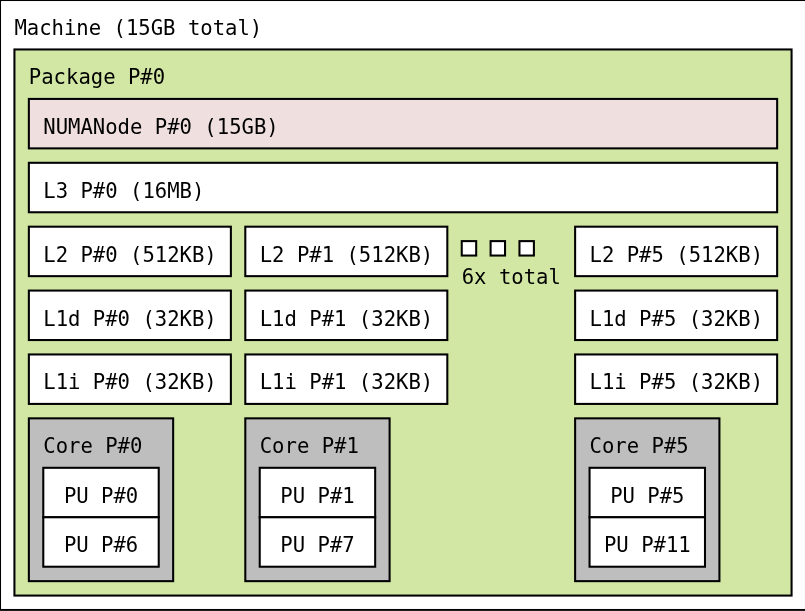
\includegraphics[width=0.8\textwidth]{./image.png}
    \caption{Sistema utilizado 6 núcleos.}
    \label{fig:mi_imagen}
\end{figure}

\section{Ejercicios}

\begin{enumerate}
	\item \textbf{Cuestión 1.} Justificar qué funciones y/o zonas del código son paralelizables. No es necesario indicar las directivas OpenMP que sería necesario utilizar.


	
\item \textbf{Cuestión 2.} Con el fin de obtener un código más eficiente en la parte de memoria compartida y poder optimizar el proceso de mejora de la población de individuos: reemplazar las llamadas a la función \texttt{rand} por \texttt{rand\_r} (que es ``thread safe'' y se usará para el resto de cuestiones de la práctica) para evitar, por un lado, que se genere la misma secuencia de valores aleatorios en diferentes hilos y, por otro, que se pierda paralelismo durante la generación de dichos valores debido a la secuencialidad que introduce la función \texttt{rand}. Además, añadir el código necesario para implementar correctamente la generación aleatoria a lo largo del algoritmo.

Para ello, una posibilidad sería crear en \texttt{mh.c} una variable global \texttt{seed} que se hará \texttt{threadprivate} y que se pasará como argumento por referencia a \texttt{rand\_r}. Así, además, cada hilo podrá inicializar \texttt{seed} en paralelo de forma independiente (por ejemplo, en función del tiempo del sistema, de su identificador de hilo o una combinación de ambos) en una primera región paralela situada justo antes de generar la población inicial de subconjuntos $B$ del problema MDP (bucle \texttt{for} que crea cada individuo, que identificaremos como \texttt{FOR\_INI}). Es en esta generación aleatoria de individuos donde el efecto sobre el paralelismo de \texttt{rand\_r} en lugar de \texttt{rand} es claramente apreciable.

Paralelizar el bucle \texttt{FOR\_INI}, lanzar ejecuciones y tomar tiempos, representando en una misma gráfica dos series de tiempos variando el número de hilos: serie (a) usando \texttt{rand}, y serie (b) usando \texttt{rand\_r} y las modificaciones del código previamente indicadas. Analizar los resultados obtenidos.

\item \textbf{Cuestión 3.} Paralelizar la función \texttt{fitness} utilizando, por un lado, los constructores \texttt{critical} y \texttt{atomic} (de forma independiente) y, por otro, la cláusula \texttt{reduction}, indicando en cada caso qué variables serían privadas y cuáles compartidas. Ejecutar el código variando el número de hilos y comparar los resultados obtenidos respecto a versión secuencial utilizando las métricas de rendimiento.

Justificar de forma teórica las diferencias y optimizar, en lo posible, el código de \texttt{critical} y \texttt{atomic} teniendo en cuenta cómo está implementada internamente \texttt{reduction}.

\item \textbf{Cuestión 4.} Probar diferentes formas de reparto de trabajo, \texttt{scheduling} (\texttt{static}, \texttt{dynamic}, \texttt{guided}), variando el tamaño de asignación (\texttt{chunk\_size}) en aquellos bucles en los que se considere necesario. Ejecutar el código variando el número de hilos y justificar los tiempos de ejecución y rendimiento obtenidos con cada política.

\item \textbf{Cuestión 5 (2ª Semana).} Paralelizar la función \texttt{cruzar} utilizando secciones. ¿Se podría usar la cláusula \texttt{nowait}? (argumentar la respuesta). Ejecutar el código variando el número de hilos y justificar el rendimiento obtenido.

\item \textbf{Cuestión 6.} Reemplazar las llamadas a la función \texttt{qsort} por la función \texttt{mergeSort} que se muestra, para ordenar la población por \texttt{fitness}, no para ordenar los elementos de cada individuo. A continuación, paralelizar dicha rutina mediante el uso de tareas (\texttt{OpenMP tasks}) y ejecutar el código variando el número de hilos. La función \texttt{mezclar} a la que invoca se proporciona en el fichero \texttt{mezclar.c}.

\begin{lstlisting}[style=EstiloC]
void mergeSort(Individuo **poblacion, int izq, int der)
{
    int med = (izq + der)/2;
    if ((der - izq) < 2) { return; }
    mergeSort(poblacion, izq, med);
    mergeSort(poblacion, med, der);
    mezclar(poblacion, izq, med, der);
}
\end{lstlisting}

¿Se reduce el tiempo de ejecución? Si no es así, explica las posibles causas. Estudia si para los tamaños de población que manejamos (usualmente $\le 2000$ individuos) pueden mejorar el rendimiento del algoritmo paralelo: (a) la optimización del código de la función \texttt{mezclar} respecto a la gestión de la memoria, o (b) el uso de condicionales en las directivas \texttt{task} para generar tareas hasta un cierto umbral de tamaño de la población.

\item \textbf{Cuestión 7.} Explicar para qué se usan en general, y si es necesario utilizar de forma explícita en alguna zona del código los siguientes constructores: \texttt{barrier}, \texttt{single}, \texttt{master}, \texttt{ordered}. Considerar también su posible uso en un código paralelo optimizado (como el requerido en la Cuestión 8).

\item \textbf{Cuestión 8.} Paralelizar la totalidad del algoritmo utilizando las directivas OpenMP que se considere mejor para cada función o bucle (y que pueden ser distintas a las usadas para resolver las cuestiones). Justificar las decisiones tomadas. De este modo, se pretende tener un código paralelo óptimo en memoria compartida que se podrá usar posteriormente para comparar con el código paralelo de paso de mensajes e híbrido implementado en las siguientes prácticas.

\item \textbf{Cuestión 9.} Realizar el informe final incluyendo las conclusiones generales y valoración personal sobre el trabajo realizado.
\end{enumerate}








\end{document}